   
        
        \begin{ledgroupsized}[r]{120mm}
        \footnotesize 
        \pstart        
        \noindent\textbf{\"{U}berlieferung:}  
        \pend
        \end{ledgroupsized}
      
       
              \begin{ledgroupsized}[r]{114mm}
              \footnotesize 
              \pstart \parindent -6mm
              \makebox[6mm][l]{\textit{L}}Konzept: LH XXXV 15, 6 Bl. 46, 74. 1 Bog. 2\textsuperscript{o}. 3/4 S. auf Bl. 74 v\textsuperscript{o}. Linke Spalte mit Ausnahme der oberen 8 Zeilen unser Text. Zu den verbleibenden Seiten vgl. N. 2\protect\raisebox{-0.5ex}{\tiny{1}}. Geringe Textverluste am unteren Rand durch Papierabbruch.\\KK 1, Nr. 193 B \pend
              \end{ledgroupsized}
        \vspace*{8mm}
        \pstart
        \normalsize
      [74 v\textsuperscript{o}] Instrumentum Longitudinum\protect\index{Sachverzeichnis}{longitudo} breviter tale esto: Fiat rotula aus trat, illius pennae sint ex subtilissimo blech. Incurvato aliquantum, ut ventum scilicet aerem tanto melius sinu quasi velum excipiat. Haec rotula in capsam angustam collocetur, ita ut aer in ea se diffundere non possit, et non plus spatii contineat fere, quam rota occupat. Sit aditus aeri ab una et exitus ab altera directe opposita parte, ita ut pennarum summitates sint in linea recta intus initum et exitum. Porro qua aditus aeri esse debet, fit \edtext{tubus sinum extro versus}{\lemma{fit}\Afootnote{ \textit{ (1) }\ exterius \textit{ (2) }\ tubus sinum extro versus \textit{ L}}} late expandens, interius in acumen desinens multis modis flexum et incurvatum. Exitus sinum introrsus, acumen extrorsum pandat, flexione illi non opus \edtext{dummodo}{\lemma{opus}\Afootnote{ \textit{ (1) }\ nec \textit{ (2) }\ dummodo \textit{ L}}} sit, quod a vento illabente pertegat. Esto etiam \edtext{}{\lemma{}\Afootnote{etiam \textbar\ ita \textit{ gestr.}\ \textbar\ versum \textit{ L}}}versum deorsum exeuntis acumen, ut protectum nihil impediat exitum. Haec capsula ponatur in loco aeri exposito, v.g. infigatur stylo, \selectlanguage{ngerman}wie ein wetterhahn.\selectlanguage{latin} Porro Rotam\protect\index{Sachverzeichnis}{rota} axis, sed cum rota\protect\index{Sachverzeichnis}{rota} mobilis transeat, et eam \edtext{in una parte capsulae incumbentem faciat}{\lemma{eam}\Afootnote{ \textit{ (1) }\ affigat \textit{ (2) }\ in [...] faciat \textit{ L}}}, sic tamen ut motus circa axem maneat liber. Iste axis sit tenuissima acicula. Ea ex altera parte porrigatur extra capsulam non incumbens, nisi in \edtext{loco extra capsulam post alteram}{\lemma{in}\Afootnote{ \textit{ (1) }\ altero \textit{ (2) }\ loco extra capsulam post alteram \textit{ L}}} rotam. Extra capsulam ergo similem prorsus rotam\protect\index{Sachverzeichnis}{rota} contineat, sed quo levior sit, eo discrimine, quod pinnis tam grandibus non opus, imo pro pinnis servient aciculae sibi conjuncte triquetrice hac forma, eminentes $\bigtriangleup$. Porro \edtext{illa rota sit inter duos parietes}{\lemma{Porro}\Afootnote{ \textit{ (1) }\ illi rotae\protect\index{Sachverzeichnis}{rota|textit} super incumbat \textit{ (2) }\ illa [...] parietes \textit{ L}}}, in altero averso axis ejus cum priore communis, mobilis, sit firmatus, super Rotam hanc 2\textsuperscript{dam} sit linea longa aus eisentrat, continuis sinulis similis et distantiae eminentiis, instar serrae, ut rota\protect\index{Sachverzeichnis}{rota} secunda. Haec linea praeterea habeat unam longam aciculam descendentem. Porro haec linea quovis quadrante horae demittatur a portatoribus rigidis \protect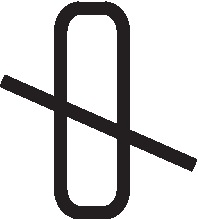
\includegraphics[width=0.04\textwidth]{images/74vIL} duobus, quorum lineae rigidae incedant intra incisuras in pariete utroque, et descendant infra rotam\protect\index{Sachverzeichnis}{rota}, et lineam serratam relinquant in rota\protect\index{Sachverzeichnis}{rota} ab ea propellendam, postea tanto tempore, quanto sinet \edtext{[quater]}{\Afootnote{quatuor\textit{\ L \"{a}ndert Hrsg. }}} quadrans ibi relinquentes resurgant rursus et reattollant. Post ultimum quadrantem \edtext{horae}{\lemma{}\Afootnote{horae \textit{ erg.} \textit{ L}}}, postquam resublata fuerit linea serrata haec contingat. Sit in linea serrata ea longa acus\protect\index{Sachverzeichnis}{acus} non firmata sed supra eam in alia parallela linea aus trat simili simplice. Dum igitur propellitur a rota\protect\index{Sachverzeichnis}{rota} secunda linea serrata, propellitur simul et simplex superius parallela, quippe quia acu connexae sunt. Postquam vero a quadrante ultimo relevata sit linea serrata \edtext{(acicula}{\lemma{(}\Afootnote{ \textbar\ nam \textit{ gestr.}\ \textbar\ acicula \textit{ L}}} cum ea non descendit) tunc superius malleoli duo utrinque a latere utroque hypomochlii (hypomochlium autem habebit foramen ut per [id]\edtext{}{\Afootnote{eam\textit{\ L \"{a}ndert Hrsg. } }} libere transire \edtext{possit}{\lemma{}\Afootnote{possit \textit{ erg.} \textit{ L}}}, et sit tale ut ad mallei ictum cedat et ipsum, et descendat aliquantulum) pulsent lineam simplicem, et ita descendet acus, et pulsabit inferius chartam, et ei foramen imprimet. Charta inferius subjecta sit \edtext{sed}{\lemma{sit}\Afootnote{ \textit{ (1) }\ loco \textit{ (2) }\ sed \textit{ L}}} sic ut sub rotam\protect\index{Sachverzeichnis}{rota} directe non veniat. Sit autem \edtext{}{\lemma{}\Afootnote{autem \textbar\ v.g. \textit{ gestr.}\ \textbar\ der \textit{ L}}}\selectlanguage{ngerman}der Ramen, darein der papyr komt\selectlanguage{latin} compactus ex aciculis ferreis, et latus septentrionale habent eminentes plurimas aciculas omnes fortiter polo\protect\index{Sachverzeichnis}{polus} magnetis\protect\index{Sachverzeichnis}{magnes} versus arcton inclinaturo affrictas, oppositae opposito. De caetero latera quasi caudicata quatuor circuitus linearum conjungantur similibus subtilissimis aciculis cum fulcro cui incumbunt. Fulcrum sit acies similiter tenuis \selectlanguage{ngerman}wie im compas\protect\index{Sachverzeichnis}{Kompass}\selectlanguage{latin} descendens inferius ita ut neque sursum neque deorsum moveri, libere tamen circumagi possit. Quod facile praestitu. \edtext{Jam in}{\lemma{praestitu.}\Afootnote{ \textit{ (1) }\ Ea ratione in \textit{ (2) }\ Jam in \textit{ L}}} 4 angulis des Ramens emineant sursum aciculae, his infigatur charta firma, sed levis. Jam charta cum ramen semper se collocabit in situm ad polos\protect\index{Sachverzeichnis}{polus}, quomodocunque vertatur navis\protect\index{Sachverzeichnis}{navis}. Et ita impressione aciculae superioris \edtext{progredientis}{\lemma{superioris}\Afootnote{ \textit{ (1) }\ et ea \textit{ (2) }\ progredientis \textit{ L}}} perfecte tum celeritas\protect\index{Sachverzeichnis}{celeritas} tum flexio navis\protect\index{Sachverzeichnis}{navis} apparebit. Uno ergo nondum explicatum horologium\protect\index{Sachverzeichnis}{horologium}, quod quovis quadrante demittat et attollat portatores et quavis hora malleolo percutiat lineam simplicem. Quod cuivis artifici praestare proclive. Debet vero qualibet septimana nova charta attigi priore demta, et horologium\protect\index{Sachverzeichnis}{horologium} readduci \edtext{cum linea serrata}{\lemma{}\Afootnote{cum linea serrata \textit{ erg.} \textit{ L}}} seu reconstitui. \edtext{Idque}{\lemma{reconstitui.}\Afootnote{ \textit{ (1) }\ Ita \textit{ (2) }\ Idque \textit{ L}}} ne tempore minus congruo fiat, illud horologium\protect\index{Sachverzeichnis}{horologium} simul horas sonet, aut si non placet, saltem tempore decursus prope finem insolite strepat. Et machina sit locata prope compas\protect\index{Sachverzeichnis}{Kompass}, ne oblivione transmittatur.\pend 